\documentclass[12pt,a4paper]{book}

% ---------- Encoding and language ----------
\usepackage[utf8]{inputenc}
\usepackage[T1]{fontenc}
\usepackage[english]{babel}

\usepackage{xcolor}

% ---------- Page layout ----------
\usepackage[a4paper,margin=2.5cm]{geometry}
\usepackage{setspace}
\onehalfspacing

% ---------- Math packages ----------
\usepackage{amsmath,amssymb,amsthm,mathtools}
\usepackage{tikz}
\usetikzlibrary{positioning, shapes.geometric, calc}
\usepackage{algorithm}
\usepackage{algpseudocode}
\usepackage{subcaption}
\usepackage{tabularx}
\usepackage{chngcntr}
% \counterwithout{table}{chapter}
% \counterwithout{algorithm}{chapter}
 
\usepackage{booktabs}
\usepackage{ragged2e}
\usepackage{siunitx}
\sisetup{
    table-number-alignment = center,
    table-format = 1.3, % one digit before decimal, three after
}

% ---------- Theorem environments ----------
\theoremstyle{plain}
\newtheorem{theorem}{Theorem}[chapter]
\newtheorem{lemma}[theorem]{Lemma}
\newtheorem{proposition}[theorem]{Proposition}
\newtheorem{corollary}[theorem]{Corollary}
 
\theoremstyle{definition}
\newtheorem{definition}[theorem]{Definition}
\newtheorem{example}[theorem]{Example}
 
\theoremstyle{remark}
\newtheorem{remark}[theorem]{Remark}

% ---------- Useful custom commands ----------
\newcommand{\R}{\mathbb{R}}
\newcommand{\N}{\mathbb{N}}
\newcommand{\Z}{\mathbb{Z}}
\newcommand{\Q}{\mathbb{Q}}
\newcommand{\C}{\mathbb{C}}
\newcommand{\eps}{\varepsilon}
\newcommand{\diag}{\mathrm{diag}}
\newcommand{\dlatent}{d_{\mathrm{latent}}}
\newcommand{\dhidden}{d_{\mathrm{hidden}}}

% ---------- Title and author ----------
\title{Mathematical Notes}
\author{Your Name}
\date{\today}

% ---------- Document ----------
\begin{document}


% \maketitle
% \tableofcontents
% \bigskip
\chapter{isudbvisuf}

\cite{Demmel1983}
\begin{definition} % Wilkinson
    Let $T \in \C^{d\times d}$. We say that $T$ is defective if its Jordan canonical form is not strictly diagonal, i.e., if there exists a non-trivial Jordan block (of dimension $>1$). Equivalently, $T$ has fewer than $d$ linearly independent eigenvectors.
\end{definition}
\begin{definition}
    For a matrix $T \in \C^{d \times d}$, we define the distance to the nearest defective matrix as:
    $\delta(T) := \inf \{\,\|A - T\| \, : \, A \in \C^{d \times d} \text{ and } A \text{ is defective }\}$.
\end{definition}

\begin{theorem}[Schur]
    Let $T\in\C^{d\times d}$ and let $\sigma(T) = \left(\lambda_1, \dots, \lambda_d\right)$ denote its spectrum (with multiplicities counted) in an arbitrary order. Then there exists a unitary matrix $Q$ and an upper-triangular matrix $U$, such that $T = Q^*UQ$ and $\mathrm{diag}(U) = \left(\lambda_1, \dots, \lambda_d\right)$.
\end{theorem}
\begin{proof}
    See \cite[p. 79]{HornJohnson1985}.
\end{proof}


\begin{lemma}\label{lemma} % Demmel lemma 2.1
    Let $\| \cdot \|$ denote either the Frobenius norm or the operator 2-norm on $\C^{d\times d}$. Let $P$ be a property depending only on Jordan canonical form of a matrix. For $T_0 \in \C^{d\times d}$ and a non-singular $S \in \C^{d \times d}$ define $\delta := \inf_{T \text{ satisfies } P}  \|T_0 - T\|$ and $\delta_S := \inf_{T \text{ satisfies } P} \|S^{-1}T_0S - T\|$. Then,
    \begin{equation*}
        \frac{\delta}{\kappa(S)} \leqslant \delta_S \leqslant \delta\kappa(S).
    \end{equation*}
\end{lemma}
\begin{proof}
    The property $P$ depends only on the Jordan canonical form of the matrix, therefore $T$ satisfies $P$ if and only if $S^{-1}TS$ satisfies $P$ for arbitrary non-singular matrix $S$. Using \eqref{eq:matrix-norm-inequality} and the definition of $\kappa(S)$, we get:
    \begin{equation*}
        \left\|S^{-1} T_0 S - S^{-1} T S \right\| \leqslant \left\|S^{-1}\right\| \left\|T_0 - T\right\| \left\|S\right\| = \|T_0-T\|\kappa(S).
    \end{equation*}
    This proofs the second equality. The first one can be shown analogously.
\end{proof}
\begin{theorem}
Let $T \in \C^{d \times d}$ and $\sigma(T) = (\lambda_1, \dots, \lambda_d)$ be the spectrum of $T$ (with multiplicities counted). Then: 
\begin{equation*}
    \delta(T) \leqslant \min_{i\neq j} |\lambda_i - \lambda_j|.
\end{equation*}
\end{theorem}
\begin{proof}
    Without loss of generality, assume $\min_{i\neq j} |\lambda_i - \lambda_j| = |\lambda_1 - \lambda_2| =: \varepsilon$. We will show that $\delta(T) \leqslant \varepsilon$. 
    
    Let $T = Q^T U Q$ be the Schur decomposition of $T$ such that $\mathrm{diag}(U) = (\lambda_1, \lambda_2, \dots, \lambda_d)$. Define $U' = \left(U'_{i,j}\right)_{i,j=1}^d$ by: 
    \begin{equation*} 
        U'_{i,j} = \begin{cases}
            \lambda_1, \quad \text{if } i=j=2 \\
            U_{i,j}, \quad \text{else}
        \end{cases}.
    \end{equation*}
   In other words, $U'$ is obtained from $U$ by replacing $\lambda_2$ with $\lambda_1$ on the diagonal. Set $T' := Q^* U' Q$. Since $Q$ is unitary and $\kappa(Q) = 1$, Lemma \ref{lemma} gives $\| T - T' \| \leqslant \kappa(Q) \cdot \|U - U'\| \leqslant \varepsilon $.
    
     The matrix $T'$ has a multiple eigenvalue $\lambda_1$. Let $T' = S^{-1} J S$ be its Jordan canonical form. If $T'$ is already defective at $\lambda_1$, we are done. Otherwise, $J$ contains at least two $1 \times 1$ Jordan blocks corresponding to eigenvalue $\lambda_1$. We choose $\eta > 0$ and construct $J'$ by replacing those two blocks with a non-trivial $2\times2$ Jordan block with $\eta$ on the superdiagonal:
     \begin{equation*}
         J' = \begin{pmatrix}
         \ddots & & & \\
         & \lambda_1 & \eta & \\
         & & \lambda_1 & \\
         & & & \ddots
         \end{pmatrix}.
     \end{equation*}
     Let $T'':=S^{-1}J'S$. By Lemma \ref{lemma}, $\|T' - T''\| \leqslant \|J - J'\|\cdot\kappa(S) \leqslant \eta \cdot\kappa(S)$, and by construction, $T''$ is defective.

     Thus, we have obtained a defective matrix in a $(\varepsilon + \eta \cdot \kappa(S))$-neighbourhood of $T$. Since $\eta$ was arbitrary, the desired inequality follows.
    
\end{proof}

% ---------- Title and author ----------

\chapter{Numerical experiments}
\section{Recognition of eigenvalue geometric multiplicity using a feed-forward neural network}

The aim of this experiment was to asses the ability of a neural network to recognize the geometric multiplicity of an eigenvalue. We considered a simple classification task on set of real $d\times d$ matrices with a single, non-zero eigenvalue $\lambda$ of algebraic multiplicity $d$. The goal was to classify the matrices by the geometric multiplicity of that eigenvalue. Due to homogeneity of eigenvalues, we set $\lambda = 1$ without loss of generality.

\subsection*{Experiment description}

We conducted multiple experiments, varying the categories of matrices used in the training and testing datasets, as described in the Table \ref{table:change-of-base-types}. The datasets consisted of matrices of the form:
\begin{equation}\label{eq:T_form}
    T = S^{-1}(J+\Delta)S,
\end{equation}
where $S$ is a random change-of-basis matrix (see Table \ref{table:change-of-base-types}), $\Delta$ is a random perturbation matrix with iid entries sampled from $\mathcal{N}(0, \eps)$ or zero matrix  and $J = \diag(J_1, \dots, J_g)$ is a Jordan matrix with blocks $J_1, \dots, J_g$ for eigenvalue $\lambda$ with sizes summing up to $d$. We refer to $\eps$ as the perturbation magnitude.

Matrices in random, integer, upper, lower and orthonormal datasets were exactly (up to numerical precision) matrices with one eigenvalue of algebraic multiplicity $d$ and geometrical multiplicity $g$, corresponding to the class in the task. 

In the perturbed dataset, Jordan matrices were first perturbed by a small random matrix and then transformed to a different basis. Consequently, they are only in some neighbourhood of the matrices corresponding to their respective classes. For the numerical stability, we enforced the constraint $\kappa(S) \leqslant 10^5$.

% TODO: Tu można ewentualnie dorzucić odwołanie do części pracy z oszacowaniami na te odległości z Demmela 


\begin{table}[htbp]
\centering
\begin{tabular}{
    l
    >{\RaggedRight\arraybackslash}p{0.48\textwidth}
    >{\RaggedRight\arraybackslash}p{0.30\textwidth}
}
\toprule
\textbf{Dataset} & \textbf{Description} & \textbf{Implementation details} \\
\midrule
\texttt{random} &
$S$ is a reshaped random vector sampled from $\mathcal N\left(0,I\right)$. &
\texttt{numpy.random.randn()} \\ \midrule
%
\texttt{integer} &
Entries of $S$ are sampled from a discrete uniform distribution over $\{0, \dots, 99\}$. &
\texttt{numpy.random.randint()} \\\midrule
%
\texttt{upper} &
$S$ is an upper‐triangular matrix with entries sampled from $\mathcal N\left(0,I\right)$. &
\texttt{numpy.triu(), numpy.random.randn()} \\\midrule
%
\texttt{lower} &
$S$ is a lower‐triangular matrix with entries sampled from $\mathcal N\left(0,I\right)$. &
\texttt{numpy.tril(), numpy.random.randn()} \\\midrule
%
\texttt{orthonormal} &
$S$ is an orthonormal matrix obtained via QR decomposition of a random matrix. &
\texttt{numpy.linalg.qr(), numpy.random.randn()} \\\midrule
%
\texttt{perturbed} &
The Jordan matrix $J$ is perturbed by $\Delta$ before the basis change; Perturbation magnitude $\eps=0.01$; $S$ is sampled as in the \texttt{random} dataset. &
\texttt{numpy.random.randn()} \\\midrule
%
\texttt{full} &
Union of all above datasets. &
\\
\bottomrule
\end{tabular}
\caption{Categories of change-of-basis matrices $S$ used in the experiment}
\label{table:change-of-base-types}
\end{table}


%\begin{algorithm}[h]
%
%    \begin{algorithmic}
%        \State \textbf{Input: } $\lambda$ -- eigenvalue, $g$ -- geometric multiplicity; $d$; dataset name
%         \State $J_1, J_2, \dots, J_g \gets$ Jordan blocks for eigenvalue $\lambda$ with sizes summing up to $d$
%         \State $J \gets \diag\left(J_1, J_2, \dots, J_g\right)$
%        \If{dataset is \texttt{perturbed}}
%            \State $\Delta \gets$ random perturbation matrix
%            \State $J \gets J + \Delta$
%        \EndIf
%         \State $S \gets$ random change-of-basis matrix (see Table \ref{table:change-of-base-types})
%         \State $T \gets S J S^{-1}$
%         \State \textbf{Output: } $T$
%    \end{algorithmic}
%    \caption{Matrix generation with a prescribed geometric multiplicity $g$}
%     \label{alg:random_matrix_given_g}
% \end{algorithm}


Note that in the case $g=d$, the matrix $T$ becomes simply $\lambda I$ (or $\lambda I$ with a small perturbation in the \texttt{perturbed} dataset). Distinguishing this class from the others, where $T$ is a full matrix, is trivial. Therefore we exclude class $g=d$ of diagonalizable matrices from the test set used for scoring. Nevertheless, we retain it in the training dataset to preserve balance in representations of all classes. The accuracy score of the model is defined as:
\begin{equation*}
    \text{accuracy} = \frac{\text{number of correctly classified matrices}}{\text{size of the dataset}}.
\end{equation*}

We conducted the experiments for the case $d=5$. For each experiment, except when using \texttt{full} dataset, the training dataset contained 250{,}000 matrices, i.e., 50{,}000 matrices per each geometric multiplicity $g=1,\dots,d$. For training on the \texttt{full} dataset we used 1{,}500{,}000 matrices, evenly distributed across classes and dataset types from Table \ref{table:change-of-base-types}: 50{,}000 matrices per class and type. In every trained model, $20\%$ of the training set was used as a validation set. The test datasets contained 1000 matrices per class. 

\subsection*{Model}
As the model, we employed a feed-forward deep neural network consisting of an input layer, seven fully-connected hidden layer with 256 neurons each and ReLU activation, and a final output layer. A network of this size and architecture (differing only in the input layer) achieves $97\%$ accuracy on the MNIST dataset. 

Training was performed using the Adam optimizer with learning rate $10^{-3}$ and early stopping monitoring the validation loss. Across all experiments, the training terminated after at most 13 epochs. Since the loss decreased at a similar rate on both the training and validation sets, with no signs of overfitting, we did not employ network regularization techniques, such as dropout or normalization.

\subsection*{Results}
The scores obtained in the experiments are presented in Table \ref{table:results-ex1}. We observe significant differences in performance across the various categories of training and testing matrices. This indicates structure discrepancies between matrices in datasets. 

\begin{table}[htbp]
\centering
\begin{tabular}{l S S S S S S S}
\toprule
\textbf{Test dataset} &
\multicolumn{7}{c}{\textbf{Train dataset}} \\
\cmidrule(lr){2-8}
 & \texttt{random} 
 & \texttt{integer} 
 & \texttt{upper}
 & \texttt{lower }
 & \texttt{orthon.} 
 & \texttt{perturbed} 
 & \texttt{full}\\
\midrule

% np.random.randn()
\texttt{random}      &0.531	&0.353&	0.254	&0.262	&0.283	&0.520 &0.656 \\
\texttt{integer}     &0.472	&0.615&	0.255	&0.259	&0.253&	0.476&  0.670\\
\texttt{upper}      & 0.465	& 0.334& 	0.865&	0.594&	0.290&	0.439 & 0.824\\
\texttt{lower}       &0.400	& 0.319&	0.361&	0.848&	0.262&	0.389&0.698 \\
\texttt{orthonormal} & 0.759 &	0.409&	0.274	&0.322	&1.000&	0.851&0.997 \\
\texttt{perturbed}   & 0.521 &	0.352&	0.259&	0.271&	0.289&	0.537& 0.611\\
\bottomrule
\end{tabular}

\caption{Accuracy scores of the models (trained on the dataset specified by each column) evaluated on different test datasets (rows).}
\label{table:results-ex1}
\end{table}

Models trained on the \texttt{random} or \texttt{integer} datasets exhibit similar behaviour across the test sets. They perform well on random cases that resemble their training data, but struggle in more specific cases, such as matrices whose Jordan canonical form is reached via triangular or orthogonal change-of-basis matrices.

Classes of matrices with triangular change-of-basis matrices $S$, collected in the \texttt{upper} and \texttt{lower} datasets, are recognized with very high accuracy by models trained on matrices of the same category. However, they are classified significantly worse by models trained on different datasets. Moreover, matrices matrices from these categories form a very limited representation of the whole space of matrices under consideration. This is reflected in the very low accuracy score achieved by models trained on \texttt{upper} or \texttt{lower} dataset when evaluated on different sets. Since we consider classification on test datasets with four classes, an accuracy of $0.25$ corresponds to the performance of a random classifier.

Consider now the models trained on the \texttt{orthonormal} dataset of matrices, where all matrices can be decomposed into their Jordan canonical form using orthogonal change-of-basis matrices; that is, their generalized eigenvectors constitute an orthonormal basis of the vector space. The neural network perfectly recognizes all geometric multiplicities within this category, but its performance on other datasets is close to random. Conversely, none of the models trained on matrices with non-orthogonal transformation matrices $S$, performs well on the \texttt{orthonormal} test set.

The final model was trained on the union of the datasets described above. It exhibits high accuracy across all test cases, only on some of them slightly lower than the score of models trained specifically on the corresponding dataset. This demonstrates that training the neural network on a sufficiently diverse and representative dataset can mitigate the weaknesses observed in previous models when evaluated on specific matrix categories.

\textcolor{red}{/ Tak naprawdę ciekawe przypadki to random--perturbed oraz perturbed--random. Tu trzeba dobrze pomyśleć, co wyszło i opisać. $\longrightarrow$ plik \texttt{.ipynb} /}

\subsection*{Impact of $\kappa(S)$ range in training and test sets on prediction quality}

Additionally to described division of change-of-basis $S$ matrices into classes, we considered the impact of condition number of $S$ in both training and test set onto model accuracy. 

The training set consisted of matrices of the form \eqref{eq:T_form} with $\Delta = 0$. Using SVD we controlled $\kappa(S)$ in the dataset, which was log-uniformly distributed, i.e., $\log\kappa(S) \sim U(\log\kappa_{\min}, \log\kappa_{\max})$. We trained two models using same hyperparameters as above, $\kappa_{\min} = 1$, $\kappa_{\max} = 100$ resp. $\kappa_{\max} = 1000$ and 50,000 matrices per each possible geometric multiplicity. 

We tested both models on multiple test sets with constant condition number across one set and varying $\kappa(S)$ between $1$ and $10^5$. For perturbation matrices $\Delta$ we used magnitude $\eps=0.01$ as well as no perturbation, $\Delta = 0$. The comparison of the results are in the Figure \ref{fig:jordan_4a}.

\begin{figure}[htbp]
    \centering
    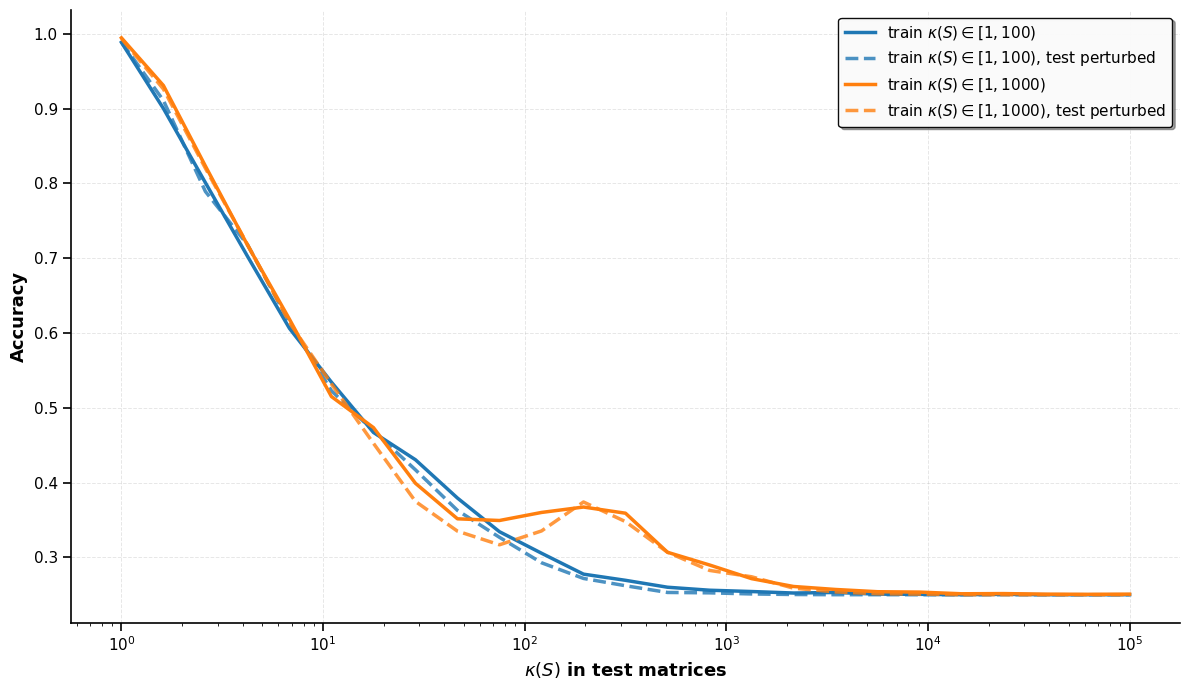
\includegraphics[width=0.9\linewidth]{images/jordan_4a.png}
    \caption{Blue lines represent accuracy of the model trained on matrices with $\kappa(S) \in [1, 100)$, whereas orange lines of the model trained on matrices with $\kappa(S) \in [1, 1000)$. Matrices in test set were not perturbed in case of continuous lines and perturbed in dashed lines.}
    \label{fig:jordan_4a}
\end{figure}    

In the interval $\kappa(S) \in (10^2, 10^3)$ we observe difference in model's prediction accuracy. This is the evidence that range of $\kappa(S)$ in the training dataset has direct impact on the performance of the model.

\section{Recognition of largest Jordan-block size of a matrix with transformer architecture}

Accuracy and training cost of the model described in previous section is not satisfactory, even for low-dimensional problem we considered. The scalability of the model is vague. For this reason, in this section we introduce another model recognizing size of the largest Jordan block of a matrix notable for higher prediction quality and better scalability. Its core modules are dimension-independent making extension onto higher dimensions possible with low training effort.

\subsection*{Problem description }
We consider matrices $T$ of the form \eqref{eq:T_form} with $J$ Jordan-matrix with one eigenvalue $\lambda\in\R$, $S$ sampled from multivariate standard normal distribution, but with constraint $\kappa(S) \leqslant 10^5$, perturbation $\Delta$ with perturbation magnitude $\eps$. The category we aim to predict of the matrix $T$ is size $m$ of the largest block in $J$.

For a true category $m_{\mathrm{true}} \in \{1, \dots d\}$ and a perturbation magnitude $\eps > 0$ we define soft-target distribution $q_{m_{\mathrm{true}}, \eps}$ over the classes $\{1, \dots d\}$. If the perturbation is neglible $\eps \leqslant\eps_0$, the distribution is a one-hot encoding; otherwise it follows a discrete Gaussian-like kernel:
\begin{equation}\label{eq:soft-target}
    q_{m_{\mathrm{true}}, \eps}(i) = \begin{cases}
        \delta_{i, m_{\mathrm{true}}}, & \text{if} \, \eps \leqslant \eps_0, \\
        \frac{\exp\left( - \frac{(i - m_{\mathrm{true}})^2}{2\tau^2} \right)}{\sum_{j=1}^d \exp\left( - \frac{(j - m_{\mathrm{true}})^2}{2\tau^2} \right)}, & \text{otherwise}
    \end{cases},
\end{equation}
where the temperature $\tau$ scales logarithmically with the perturbation:
\begin{equation*}
\tau = C \ln\left(1 + \frac{\eps}{\eps_0}\right).
\end{equation*}
We set $\eps_0 = 10^{-8}$ and $C=0.1$. This formulation ensures that as $\eps$ increases, the target distribution diffuses symmetrically around $m_{\mathrm{true}}$, reflecting higher uncertainty for larger perturbations. Conversely, as $\eps \to \eps_0^+$, the distribution sharpens toward the true class.


\subsection*{Model}
As features to the model we use powers of the shifted matrix: $N := T - \lambda I \in \R^{d \times d}$. The input is the sequence $(N, N^2, \dots, N^r)$, where $r := \mathrm{rank}(N)$ (or one-element sequence $(N)$, if $r = 0$). Note that in theory, analysis of the ranks of all matrices in the sequence, would allow us to determine full Jordan structure of the matrix $T$. 

In our implementation, we determined the rank of a matrix following numerical algorithm described in \cite{Press2007}, which corresponds to NumPy or Matlab implementation of the matrix rank. It identifies rank deficiency as number of singular values under the threshold given by formula $\sigma_1 \cdot \max(m, n)\cdot \eps_m$, where $\sigma_1$ denotes the largest singular value and $\eps_m$ denotes the data type accuracy.

First, we encode the input sequence into latent space $\R^{d_\mathrm{latent}}$ with $d_\mathrm{latent}=32$, using simple fully connected feed-forward architecture with three hidden layers, $d_{\mathrm{hidden}}=128$ neurons each, and ReLU activation after each hidden layer. We denote the encoder as mapping $E_d : \R^{d \times d} \rightarrow \R^{d_\mathrm{latent}}$ and encoded embedding $y_k := E_d(N^k)$. We map all entries in the input using the same encoder, but each dimension $d$ requires its own encoder.

As the core of the model we employ a Transformer introduced in \cite{Attention}. This attention-based mechanism is suitable for processing sequences of vectors, initially introduced for natural language processing purposes. In our implementation we used architecture with 2 layers, feed-forward nets of dimension $d_{\mathrm{hidden}}$ and 4 attention heads. After the Transformer layer we use mean pooling and obtain $\bar{z} = 1/r \sum_{i=1}^r z_i \in \R^{m}$, where $(z_1, \dots, z_r)$ is the Transformer output. In our model the Transformer is fully independent of input matrix dimension $d$ and is shared for all considered dimensions. 

The vector $\bar{z}$ is then pulled into a dimension-dedicated Classifier $C_d : \R^{\dlatent} \rightarrow \R^d$, which is a simple feed-forward fully connected neural network with one 128-dimensional hidden layer. The output is $d$-dimensional vector of logits. Applying softmax gives predicted distribution $\hat{q}$ over all possible $d$ block sizes.

The model architecture is presented in Figure \ref{fig:JordanNet}. Table \ref{table:JordanNet_weights} summarizes model size.


\begin{figure}[htbp]
    \centering
    \begin{tikzpicture}[
        % node distance: vertical=1.1cm, horizontal=0.5cm (reduced from 0.9cm)
        node distance=1.1cm and 0.5cm,
        every node/.style={font=\small},
        data/.style={draw, rounded corners, fill=gray!15,
                     minimum width=0.7cm, minimum height=1.3cm},
        pool/.style={draw, rounded corners, fill=gray!15,
                     minimum width=0.9cm, minimum height=1.4cm},
        classifier/.style={draw, rounded corners, fill=orange!25,
                           minimum width=0.9cm, minimum height=2.0cm},
        transformer/.style={draw, rounded corners, fill=blue!20,
                            minimum width=1.3cm, minimum height=7.5cm}, 
        arrow/.style={->, thick},
        encoder/.style={
            draw, trapezium, trapezium angle=75,
            shape border rotate=270,
            fill=orange!25,
            rounded corners,
            minimum width=1.5cm,
            minimum height=0.9cm
        }
    ]
    
    % --- Inputs ---
    \node[data] (N1) {$N^1$};
    \node[data, below=of N1] (N2) {$N^2$};
    \node[below=1.2cm of N2] (dots_input) {\vdots}; 
    \node[data, below=1.2cm of dots_input] (Nr) {$N^r$};
    
    % --- Encoders ---
    \node[encoder, right=of N1] (E1) {Encoder};
    \node[encoder, right=of N2] (E2) {Encoder};
    \node[below=1.4cm of E2] (dots_enc) {\vdots}; 
    \node[encoder, right=of Nr] (Er) {Encoder};
    
    % --- y outputs ---
    \node[data, right=of E1] (y1) {$y_1$};
    \node[data, right=of E2] (y2) {$y_2$};
    \node[below=1.2cm of y2] (dots_y) {\vdots}; 
    \node[data, right=of Er] (yr) {$y_r$};
    
    % --- Right Side (Vertically Centered) ---
    \coordinate (centerpoint) at ($(y1.east)!0.5!(yr.east)$);
    
    % Reduced the manual gap to the Transformer (1.2cm -> 0.8cm)
    \node[transformer, right=0.8cm of centerpoint] (T) {\rotatebox{90}{Transformer}};
    \node[pool, right=of T] (MP) {\rotatebox{90}{Mean pooling}};
    \node[data, right=of MP] (zb) {$\bar{z}$};
    \node[classifier, right=of zb] (C) {\rotatebox{90}{Classifier}};
    \node[data, right=of C] (L) {\rotatebox{90}{Softmax}};
    \node[data, right=of L, minimum width=0.8cm] (Q) {\rotatebox{0}{$\hat{q}$}};
    
    % --- Arrows ---
    \draw[arrow] (N1) -- (E1);
    \draw[arrow] (N2) -- (E2);
    \draw[arrow] (Nr) -- (Er);
    
    \draw[arrow] (E1) -- (y1);
    \draw[arrow] (E2) -- (y2);
    \draw[arrow] (Er) -- (yr);
    
    % Symmetrical arrows into Transformer
    \draw[arrow] (y1.east) -- (T.west |- y1.east);
    \draw[arrow] (y2.east) -- (T.west |- y2.east);
    \draw[arrow] (yr.east) -- (T.west |- yr.east);
    
    % Right side flow
    \draw[arrow] (T) -- (MP);
    \draw[arrow] (MP) -- (zb);
    \draw[arrow] (zb) -- (C);
    \draw[arrow] (C) -- (L);
    \draw[arrow] (L) -- (Q);
    
    \end{tikzpicture}
    \caption{Model architecture. Orange modules are trained for each dimension separately. Blue transformer is dimension-independent.}
    \label{fig:JordanNet}
\end{figure}

\begin{table}[htbp]
    \centering
    \small % Slightly smaller font to fit width
    \setlength{\tabcolsep}{4pt} % Reduce horizontal padding (default is 6pt)
    \renewcommand{\arraystretch}{1.3}
    \begin{tabular}{llr}
        \toprule
        \textbf{Module} & \textbf{General Formula ($d, \dhidden, \dlatent$)} & \textbf{Weights ($\dhidden=128, \dlatent=32$)} \\ 
        \midrule
        Encoder     & $\dhidden(d^2 + 2\dhidden + \dlatent + 3) + \dlatent$ & $128d^2 + 37,280$ \\ 
        Classifier  & $\dhidden(\dlatent + d + 1) + d$                      & $129d + 4,224$    \\ 
        Transformer & $24\dlatent^2 + 26\dlatent$                           & $25,408$          \\ 
        \midrule
        \textbf{Total} & \multicolumn{2}{r}{%
            $\underbrace{25,408}_{\text{Shared}} + \underbrace{128d^2 + 129d + 41,504}_{\text{Per dimension } d}$%
        } \\ 
        \bottomrule
    \end{tabular}
    \caption{Parameter counts for model components.}
    \label{table:JordanNet_weights}
\end{table}

\subsection*{Training}
Training of the model was splitted into two phases. In the first phase, we trained weights of Encoders $E_d$, Classifiers $C_d$ and the Transformer for dimensions $d = 4, 6, 9, 12, 15, 28$. Simultaneous training on multiple dimensions is necessary in order to make the Transformer universal across dimensions. In the second phase, we trained additional Encoder $E_d$ and Classifiers $C_d$ for $d=7, 13, 19, 23, 25, 33, 35$, with freezed Transformer parameters. Aim of this experiment was to test universality of the Transformer and cost of adding additional dimensions (also exceeding maximal dimension in the first phase).

In the first phase we used dataset of matrices of the form \eqref{eq:T_form} with $S$ sampled from multivariate standard normal distribution. Perturbation magnitude $\eps$ was sampled for each matrix in the dataset independently following a spike-and-log-uniform distribution, where $\eps = 0$ with probability $0.1$, and $\log\eps \sim \mathcal{U}(\log \eps_{\min}, \log \eps_{\max})$ otherwise. We used $\eps_{\min} = 10^{-16}$ and $\eps_{\max} = 10^{-2}$. The dataset contained 148,000 matrices, 2000 of each class $m \in \{1, \dots, d\}$ per each dimension. 

The second phase involved datasets containing 1000 matrices per each class $m$ and each dimension $d$. The matrices were generated in the same manor as in the first phase.

In both cases, random 20\% of the dataset was used for validation. As the loss we used average Kullback-Leibler divergence between true soft-target and model's output: $D_{KL}(q_{m_{\mathrm{true}}, \eps} \parallel \hat{q})$. For loss minimization we employed Adam algorithm with learning rate $10^{-3}$. Training process is presented in Figure \ref{fig:Jordanet_training}. First phase converged to desired tolerance $10^{-6}$ after 27 epochs.

\begin{figure}[htbp]
     \centering
     \begin{subfigure}[b]{0.49\textwidth}
         \centering
         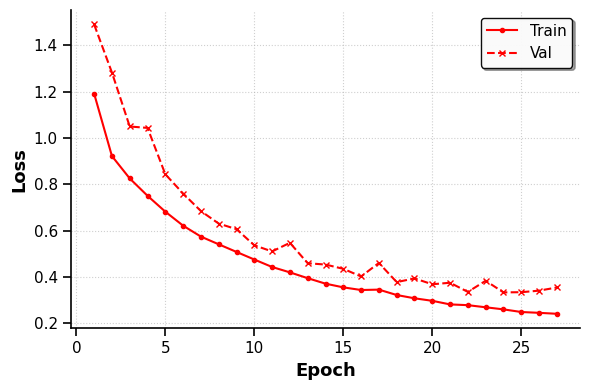
\includegraphics[width=\textwidth]{images/j8_convergence_a.png}
         \caption{First phase of training}
     \end{subfigure}
     \hfill
     \begin{subfigure}[b]{0.49\textwidth}
         \centering
         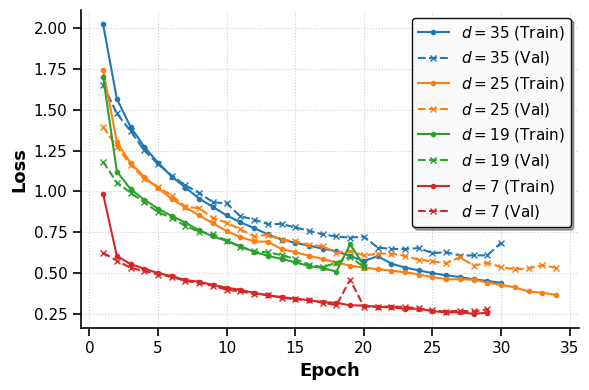
\includegraphics[width=\textwidth]{images/j8_convergence_b.png}
         \caption{Second phase of training}
     \end{subfigure}
     \caption{Loss on training and validation set during the training of the whole model (a) and of Encoders and Classifiers for additional dimensions (b). Solid lines indicate training loss, while dashed lines -- validation loss.}
     \label{fig:Jordanet_training}
\end{figure}

\subsection*{Results}
We used two quality metrics: average Kullback-Leibler divergence, analogously to training loss, and model accuracy defined as ratio of correctly recognized maximal block sizes to number all tested matrices. We assume predicted maximal block size as index, where model's output $\hat{q}$ attains highest value.

We tested the quality of predictions depending on perturbation magnitude $\eps$. For various $\eps = 0, 10^{-6}, 10^{-4}, 10^{-2}, 0.1, 1$ values and dimensions $d$ we generated test sets containing matrices of the form \eqref{eq:T_form}, 1000 matrices of each class $m$. Similarity matrices $S$ were sampled from standard normal distribution with conditioning constraint $\kappa(S) \leqslant10^5$. 

Figures \ref{fig:JordanNet_KL_loss} and \ref{fig:JordanNet_KL_accuracy} present obtained scores. \textcolor{red}{TODO....}  


\begin{figure}[htbp]
     \centering
     \begin{subfigure}[b]{0.49\textwidth}
         \centering
         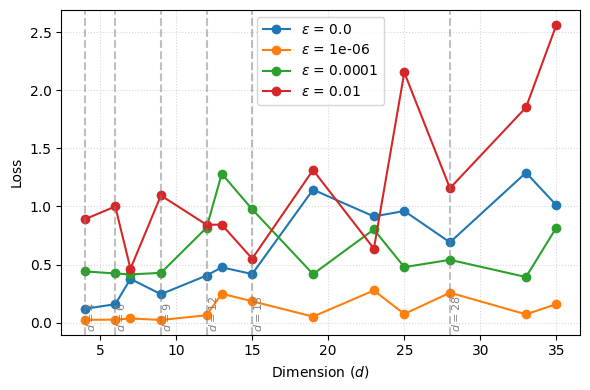
\includegraphics[width=\textwidth]{images/j8_kl_loss_a.png}
         \caption{}
     \end{subfigure}
     \hfill
     \begin{subfigure}[b]{0.49\textwidth}
         \centering
         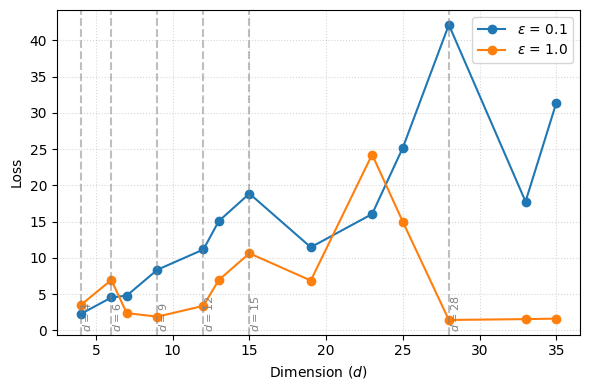
\includegraphics[width=\textwidth]{images/j8_kl_loss_b.png}
         \caption{}
     \end{subfigure}
     \caption{Average Kullback-Leibler loss per matrix depending on dimension $d$ and perturbation magnitude $\eps$. Plot (a) shows matrices with perturbations of magnitude as in training dataset, whereas plot (b) those with perturbations of larger magnitude. Dimensions involved in Transformer training are indicated by dashed grey line. }
     \label{fig:JordanNet_KL_loss}
\end{figure}

\begin{figure}[htbp]
     \centering
     \begin{subfigure}[b]{0.49\textwidth}
         \centering
         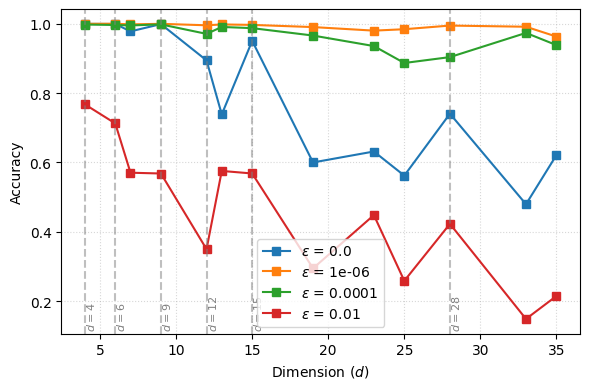
\includegraphics[width=\textwidth]{images/j8_acc_a.png}
         \caption{Full model training.}
     \end{subfigure}
     \hfill
     \begin{subfigure}[b]{0.49\textwidth}
         \centering
         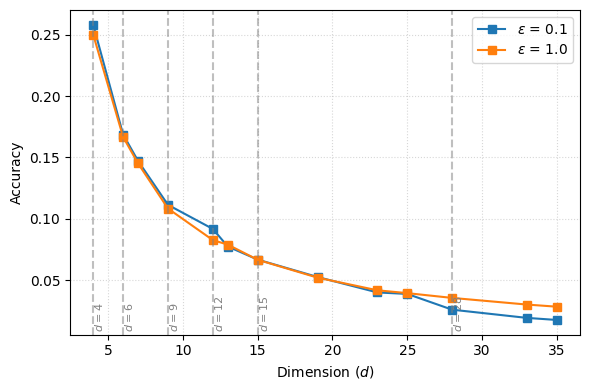
\includegraphics[width=\textwidth]{images/j8_acc_b.png}
         \caption{Training of additional dimensions.}
     \end{subfigure}
     \caption{Accuracy score depending on dimension $d$ and perturbation magnitude $\eps$. Plot (a) shows matrices with perturbations of magnitude as in training dataset, whereas plot (b) those with perturbations of larger magnitude. Dimensions involved in Transformer training are indicated by dashed grey line. }
     \label{fig:JordanNet_KL_accuracy}
\end{figure}

\begin{figure}[htbp]
    \centering
    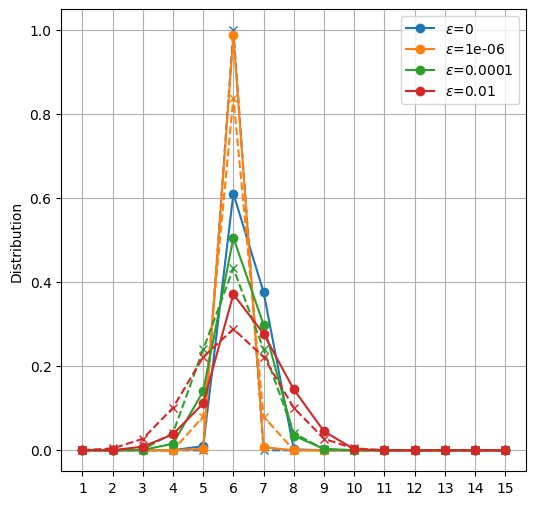
\includegraphics[width=0.5\linewidth]{images/j8_target_example.png}
    \caption{Comparison of distributions $\hat{q}$ returned by the model (solid lines) with soft-target ones $q_{m_{\mathrm{true}}, \eps}$ (dashed lines) for matrices with $d=15$, $m_{\mathrm{true}}=6$ and varying $\eps$.} 
    \label{fig:JordanNet_q_example}
\end{figure}


\bibliographystyle{abbrv}
\bibliography{bib}

\end{document}
